% =====================================================================
%  Chapter 18 — \idxw{Radar} Range-Doppler and the Fourth-Power Wall
% =====================================================================

\chapter{Radar Range-Doppler and the Fourth-Power Wall}
\label{ch:radar}

Radar\idx{Radar} is the method that answers the question this book is about most
completely. It gives the three-dimensional shape, the rotation state and the
mass, in one measurement, from a non-cooperative target, with no assumption
about convexity and none about the body's thermal behaviour. It is also the
method with the hardest physical limit in the field, and understanding that
limit is what tells you where the complementary capability has to sit.

\section{What radar measures}

A radar\idx{Radar} pulse is transmitted towards the target and its echo is received.
Three properties of the echo carry information.

The \emph{delay} between transmission and reception gives the range to the
target, and the range to each scattering element gives the depth structure.

The \emph{Doppler shift} of the echo gives the line-of-sight velocity of
each scattering element, and the velocity field gives the rotation.

The \emph{amplitude} of the echo gives the radar\idx{Radar} cross-section\idx{Radar cross-section}, which
depends on the size of the scattering elements and, in the polarimetric
case, on their shape and on the roughness of the surface. The polarimetric
signature is what distinguishes a consolidated surface from a particulate
one, and it is therefore a direct diagnostic of the density question that
Chapter 7 identified.

The combination of range and Doppler is what produces the image: the classic
delay-Doppler\idx{Delay-Doppler} inversion reconstructs a three-dimensional shape from a
two-dimensional data set, and it does so without assuming anything about the
body's convexity.

\begin{table}[!htbp]
\centering
\small
\caption{What the radar techniques deliver, and their limits.}
\label{tab:radar-methods}
\begin{tabularx}{\textwidth}{@{}P{1.24in}P{1.32in}Y@{}}
\toprule
\rowcolor{panel}
\textbf{Technique} & \textbf{Delivers} & \textbf{Constraint} \\
\midrule
Single-dish radar & range, Doppler, and a radar cross-section\idx{Radar cross-section} & needs a
radar-crossing object and a large dish \\
\rowcolor{panel}
\idxw{Bistatic radar} & range, Doppler, and a delay-Doppler\idx{Delay-Doppler} image & needs a second
station and a common view \\
\idxw{Delay-Doppler} imaging & the three-dimensional shape & the reconstruction is
ill-conditioned at low signal \\
\rowcolor{panel}
Polarimetry & the surface state, and hence a density diagnostic & the
weakest signal of the four \\
\bottomrule
\end{tabularx}
\end{table}

\section{The fourth-power wall}

The reason radar cannot characterise the catalogue is a power law, and the
exponent is what matters.

The flux of a body falls as the inverse square of its distance, so the
power it intercepts and scatters falls as \(R^{-2}\). The echo is then
spread over a solid angle that grows as \(R^{2}\), so the received power per
unit solid angle falls as \(R^{-4}\).

\begin{equation}
P_{\mathrm{recv}} \propto \frac{\sigma}{R^{4}},
\label{eq:radar4}
\end{equation}
with \(\sigma\) the radar cross-section. The fourth power is brutal. Doubling
the range divides the received power by sixteen. A radar cross-section\idx{Radar cross-section} that
is adequate at a tenth of an astronomical unit is 10,000 times weaker at
one astronomical unit.

This is the wall that shapes the whole field. More than 1,100 near-Earth
objects have been observed by radar at some point, and a few dozen have
complete radar shape models. The difference between those two numbers is the
combination of the fourth-power law\idx{Fourth-power law}, the need for a radar-crossing object,
and the reality that the dishes are on the Earth and the targets are not.

\begin{figure}[!htbp]
\centering
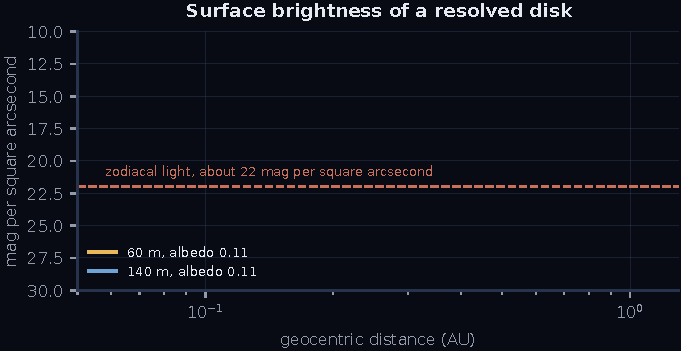
\includegraphics[width=\textwidth]{../figures/fig_brightness.pdf}
\caption{The surface brightness of a resolved disk of the 60-metre and
140-metre classes against distance, against the zodiacal background at about
22 magnitudes per square arcsecond. The lunar sky is not the constraint on
the optical channel: the target is 18 to 22 magnitudes above the
background.}
\label{fig:brightness}
\end{figure}

\section{Why the Moon does not help the radar problem, and does help the optical one}

This is where the owner's original instinct --- a ranging beam from the Moon
--- has to be handled carefully, because the instinct is right about the
physics and wrong about the comparison.

A radar system on the Moon would have a range advantage over a ground
system, and the fourth-power law\idx{Fourth-power law} means that a range advantage is worth a
great deal. But the advantage is modest in the regime that matters: for a
target at 1.3 astronomical units, the Moon's range advantage over the Earth
is only about 1.3 in the geometric sense, and the fourth-power law\idx{Fourth-power law} turns a
factor of 1.3 in range into a factor of about 2.9 in received power. That is
not nothing, but it is not the difference between characterising the
catalogue and characterising a handful of objects.

The reason is structural, and it is the reason the book puts the optical
channel rather than the radar channel at the centre of the lunar case. The
optical channel's range dependence is the inverse square of the flux law,
which is far milder, and the optical channel does not require the target to
be radar-crossing, which is a severe selection effect: only a few per cent
of small near-Earth objects have surfaces that are radar-bright enough to
detect at all.

\begin{table}[!htbp]
\centering
\small
\caption{The two channels compared, on the physics rather than on the
instruments.}
\label{tab:channels}
\begin{tabularx}{\textwidth}{@{}P{1.19in}P{1.37in}Y@{}}
\toprule
\rowcolor{panel}
\textbf{Property} & \textbf{Optical} & \textbf{Radar} \\
\midrule
Range dependence & \(R^{-2}\) on the flux & \(R^{-4}\) on the echo \\
\rowcolor{panel}
Target selection & any object bright enough & only radar-crossing objects \\
Shape & a projection, needs a model & three-dimensional, direct \\
\rowcolor{panel}
Mass & not directly & yes, from the trajectory \\
Density & no & yes, from polarimetry \\
\bottomrule
\end{tabularx}
\end{table}

The last two rows are the reason radar remains indispensable and the reason
it cannot be the answer to the catalogue: it is the only method that gives
the mass and the density, and it is the method whose reach is limited to a
small fraction of the population.

\section{Bistatic radar, and the Moon as a reflector}

Bistatic radar\idx{Bistatic radar} separates the transmitter from the receiver, and that
separation buys two things: a much larger effective baseline, and the
ability to use a body that is not a radio telescope as the transmitter or the
reflector.

The Australian record is the strongest demonstration in the field. Using the
Green Bank Telescope and the Parkes observatory as a bistatic pair, more than
fifty near-Earth objects have been characterised since 2015, including
delay-Doppler\idx{Delay-Doppler} images and polarimetric measurements.

The Moon is itself a bistatic radar\idx{Bistatic radar} reflector of a kind, and the concept has
been demonstrated: radio-occultation work has used the Moon's limb as a
diffracting edge, and the 2017 occultation of (372) Palma measured by the
Very Long Baseline Array is the most precise use of a lunar limb as an
optical element in the history of the field.

\begin{seamnote}{The pattern, and the book's use of it}
Every one of these lunar exploits uses the Moon as a passive reflector or a
diffracting edge. None of them uses the Moon as a telescope. The book follows
the same pattern: the lunar contribution is a stable baseline and a long
observing window, and the instrument that uses them is an optical
interferometer, because that is the instrument for which a kilometre-scale
stable baseline changes the answer.
\end{seamnote}

\begin{keytakeaways}
\item Radar delivers the three-dimensional shape, the spin state and the mass,
and it is the only method that answers the density question directly.
\item The received echo power falls as the fourth power of range, and that
law is the wall the field has never got past.
\item The lunar range advantage is worth about a factor of three in received
power at 1.3 astronomical units, which is real but not transformative, and
the radar selection effect is the harder constraint.
\item The lunar exploits that have worked are all passive: the Moon as a
diffracting edge and as a bistatic reflector, never as a telescope.
\end{keytakeaways}
